% AER E 361 Mission Report Template
% Spring 2023
% Template created by Yiqi Liang and Professor Matthew Nelson

% Document Configuration DO NOT CHANGE
\documentclass[12 pt]{article}
% --------------------LaTeX Packages---------------------------------
% The following are packages that are used in this report.
% DO NOT CHANGE ANY OF THE FOLLOWING OR YOUR REPORT WILL NOT COMPILE
% -------------------------------------------------------------------

\usepackage{hyperref}
\usepackage{parskip}
\usepackage{titlesec}
\usepackage{titling}
\usepackage{graphicx}
\usepackage{graphviz}
\usepackage[T1]{fontenc}
\usepackage{titlesec, blindtext, color} %for LessIsMore style
\usepackage{tcolorbox} %for references box
\usepackage[hmargin=1in,vmargin=1in]{geometry} % use 1 inch margins
\usepackage{float}
\usepackage{tikz}
\usepackage{svg} % Allows for SVG Vector graphics
\usepackage{textcomp, gensymb} %for degree symbol
\hypersetup{
	colorlinks=true,
	linkcolor=blue,
	urlcolor=cyan,
}
\usepackage{biblatex}
\addbibresource{lab-report-bib.bib}
\usepackage{amsmath}
\usepackage{listings}
\usepackage{multicol}
\usepackage{array}

\usepackage{hologo} %KYR: for \BibTeX
%\usepackage{algpseudocode}
%\usepackage{algorithm}
% This configures items for code listings in the document
\usepackage{xcolor}

\usepackage{fancyhdr} % Headers/Footers
\usepackage{siunitx} % SI units
\usepackage{csquotes} % Display Quote
\usepackage{microtype} % Better line breaks

\definecolor{commentsColor}{rgb}{0.497495, 0.497587, 0.497464}
\definecolor{keywordsColor}{rgb}{0.000000, 0.000000, 0.635294}
\definecolor{stringColor}{rgb}{0.558215, 0.000000, 0.135316}
\definecolor{mygreen}{rgb}{0,0.6,0}
\definecolor{mygray}{rgb}{0.5,0.5,0.5}
\definecolor{mymauve}{rgb}{0.58,0,0.82}

\lstdefinestyle{customc}{
  belowcaptionskip=1\baselineskip,
  breaklines=true,
  frame=L,
  xleftmargin=\parindent,
  language=C,
  showstringspaces=false,
  basicstyle=\footnotesize\ttfamily,
  keywordstyle=\bfseries\color{green!40!black},
  commentstyle=\itshape\color{purple!40!black},
  identifierstyle=\color{blue},
  stringstyle=\color{orange},
 }

 \lstset{ %
  backgroundcolor=\color{white},   % choose the background color; you must add \usepackage{color} or \usepackage{xcolor}
  basicstyle=\footnotesize,        % the size of the fonts that are used for the code
  breakatwhitespace=false,         % sets if automatic breaks should only happen at whitespace
  breaklines=true,                 % sets automatic line breaking
  captionpos=b,                    % sets the caption-position to bottom
  commentstyle=\color{commentsColor}\textit,    % comment style
  deletekeywords={...},            % if you want to delete keywords from the given language
  escapeinside={\%*}{*)},          % if you want to add LaTeX within your code
  extendedchars=true,              % lets you use non-ASCII characters; for 8-bits encodings only, does not work with UTF-8
  frame=tb,	                   	   % adds a frame around the code
  keepspaces=true,                 % keeps spaces in text, useful for keeping indentation of code (possibly needs columns=flexible)
  keywordstyle=\color{keywordsColor}\bfseries,       % keyword style
  language=Python,                 % the language of the code (can be overrided per snippet)
  otherkeywords={*,...},           % if you want to add more keywords to the set
  numbers=left,                    % where to put the line-numbers; possible values are (none, left, right)
  numbersep=8pt,                   % how far the line-numbers are from the code
  numberstyle=\tiny\color{commentsColor}, % the style that is used for the line-numbers
  rulecolor=\color{black},         % if not set, the frame-color may be changed on line-breaks within not-black text (e.g. comments (green here))
  showspaces=false,                % show spaces everywhere adding particular underscores; it overrides 'showstringspaces'
  showstringspaces=false,          % underline spaces within strings only
  showtabs=false,                  % show tabs within strings adding particular underscores
  stepnumber=1,                    % the step between two line-numbers. If it's 1, each line will be numbered
  stringstyle=\color{stringColor}, % string literal style
  tabsize=2,	                   % sets default tabsize to 2 spaces
  title=\lstname,                  % show the filename of files included with \lstinputlisting; also try caption instead of title
  columns=fixed                    % Using fixed column width (for e.g. nice alignment)
}

\lstdefinestyle{customasm}{
  belowcaptionskip=1\baselineskip,
  frame=L,
  xleftmargin=\parindent,
  language=[x86masm]Assembler,
  basicstyle=\footnotesize\ttfamily,
  commentstyle=\itshape\color{purple!40!black},
}

\lstset{escapechar=@,style=customc}

\titlelabel{\thetitle.\quad}

% From here on out you can start editing your document
\newcommand{\subtitle}[1]{%
  \posttitle{%
    \par\end{center}
    \begin{center}\LARGE#1\end{center}
    \vskip0.5em}%
}

\title{\textbf{Iowa State University
\\{\Large Aerospace Engineering}}}
\subtitle{AER E 322 Lab 7\\
		  Column Buckling}
\author{Matthew Mehrtens, Peter Mikolitis, and Natsuki Oda}

\newcommand{\etal}{\textit{et al}., }
\newcommand{\ie}{\textit{i}.\textit{e}., }
\newcommand{\eg}{\textit{e}.\textit{g}., }

% Define the headers and footers
\setlength{\headheight}{70.63135pt}
\geometry{head=70.63135pt, includehead=true, includefoot=true}
\pagestyle{fancy}
\fancyhead{}\fancyfoot{} % clears the headers/footers
\fancyhead[L]{\textbf{AER E 322}}
\fancyhead[C]{\textbf{Aerospace Structures Laboratory Summary}\\
			  \textbf{Lab 7 Column Buckling}\\
			  Section 4 Group 2\\
			  Matthew Mehrtens, Peter Mikolitis, and Natsuki Oda\\
			  \today}
\fancyhead[R]{\textbf{Spring 2023}}
\fancyfoot[C]{\thepage}

\begin{document}
\maketitle
\tableofcontents
\section{Introduction} \label{introduction}
In this lab, we studied column buckling by using the Instron machines to apply a compressive load to five different column specimens. The columns varied in shape/dimensions, material, length, and ``end-configuration''. We tested a cylindrical and rectangular aluminum column and three cylindrical steel columns. By varying the properties of the columns, we were able to make connections between the theoretical or calculated material properties and the physical behavior of columns. In doing so, we gained a better insight into static column design and analysis.

\section{Objectives} \label{objectives}
\begin{itemize}
	\item Accurately predict the force at which the sample will buckle
	\item Visually observe the column buckling and record the force at which buckling first occured
	\item Use the analysis of observations from the lab to design a new column
\end{itemize}

\section{Hypothesis} \label{hypothesis}
For the rectangular specimen, we expected the column to buckle about the axis with the lowest moment of inertia, \ie the axis with the least resistance to bending. We also expected the cylindrical aluminum column and the one-pivot-one-fixed cylindrical steel column to have the least perceptible ``jolt'' due to their relatively low slenderness ratios.

\section{Work Assignments} \label{work_assignments}
Refer to Table \ref{table:work_assignments} for the distribution of work during this lab.

\begin{table}[!htbp]
\caption{Work assignments for AER E 322 Lab 7.}
\begin{center}
	\begin{tabular}{| c | c | c | c |}
		\hline
		\multicolumn{1}{| c |}{\textbf{Task}} & \textbf{Matthew} & \textbf{Peter} & \textbf{Natsuki} \\
		\hline
		\multicolumn{4}{| c |}{\textit{Lab Work}} \\
		\hline
		Data Recording & X & X & X \\
		\hline
		Exp. Setup & X & X & X \\
		\hline
		Exp. Work & X & X & X \\
		\hline
		Exp. Clean-Up & X & X & X \\
		\hline
		\multicolumn{4}{| c |}{\textit{Report}} \\
		\hline
		Introduction & X & X & \\
		\hline
		Objectives & & X & \\
		\hline
		Hypothesis & & X & \\
		\hline
		Materials & & & X \\
		\hline
		Apparatus & & & X \\
		\hline
		Procedures & & & X \\
		\hline
		Data & X & & \\
		\hline
		Analysis & X & X & X \\
		\hline
		Conclusion & X & X & \\
		\hline
		Editing & & & \\
		\hline
	\end{tabular}
\end{center}
\label{table:work_assignments}
\end{table}

\section{Materials} \label{materials}
\begin{itemize}
	\item Five metal column specimens with specifications defined in \ref{tbl:column_specs}
	\item Instron machine (see Figures \ref{fig:instron_1} and \ref{fig:instron_2})
	\item Socket to fix the ends of the specimens in a pivot configuration (see Figure \ref{fig:socket})
	\item Ruler to measure the length of the specimen 
\end{itemize}

\begin{table}[!htbp]
\caption{The five column buckling test configurations.}
\begin{center}
	\begin{tabular}{|c|c|c|c|c|}
		\hline
		Specimen ID&Material&Cross-Section [\unit{in.}]&Length [\unit{in.}]&End Condition\\
		\hline
		I&aluminum&$\frac{3}{8}$ dia.&\num{30}&both pivot (round)\\
		\hline
		II&aluminum&\numproduct{0.25x1}&\num{30}&both pivot (round)\\
		\hline
		III&steel&$\frac{1}{4}$ dia.&\num{30}&both pivot (round)\\
		\hline
		IV&steel&$\frac{1}{4}$ dia.&\num{24}&both pivot (round)\\
		\hline
		V&steel&$\frac{1}{4}$ dia.&\num{27.5} (\num{30} original)&one pivot, one fixed\\
		\hline
	\end{tabular}
\end{center}
\label{tbl:column_specs}
\end{table}

\section{Apparatus} \label{apparatus}
See Figures \ref{fig:instron_1}, \ref{fig:instron_2}, and \ref{fig:socket} for images of the lab apparatus.

\begin{figure}[htbp]
    \centering
    \begin{minipage}{0.45\textwidth}
        \centering
		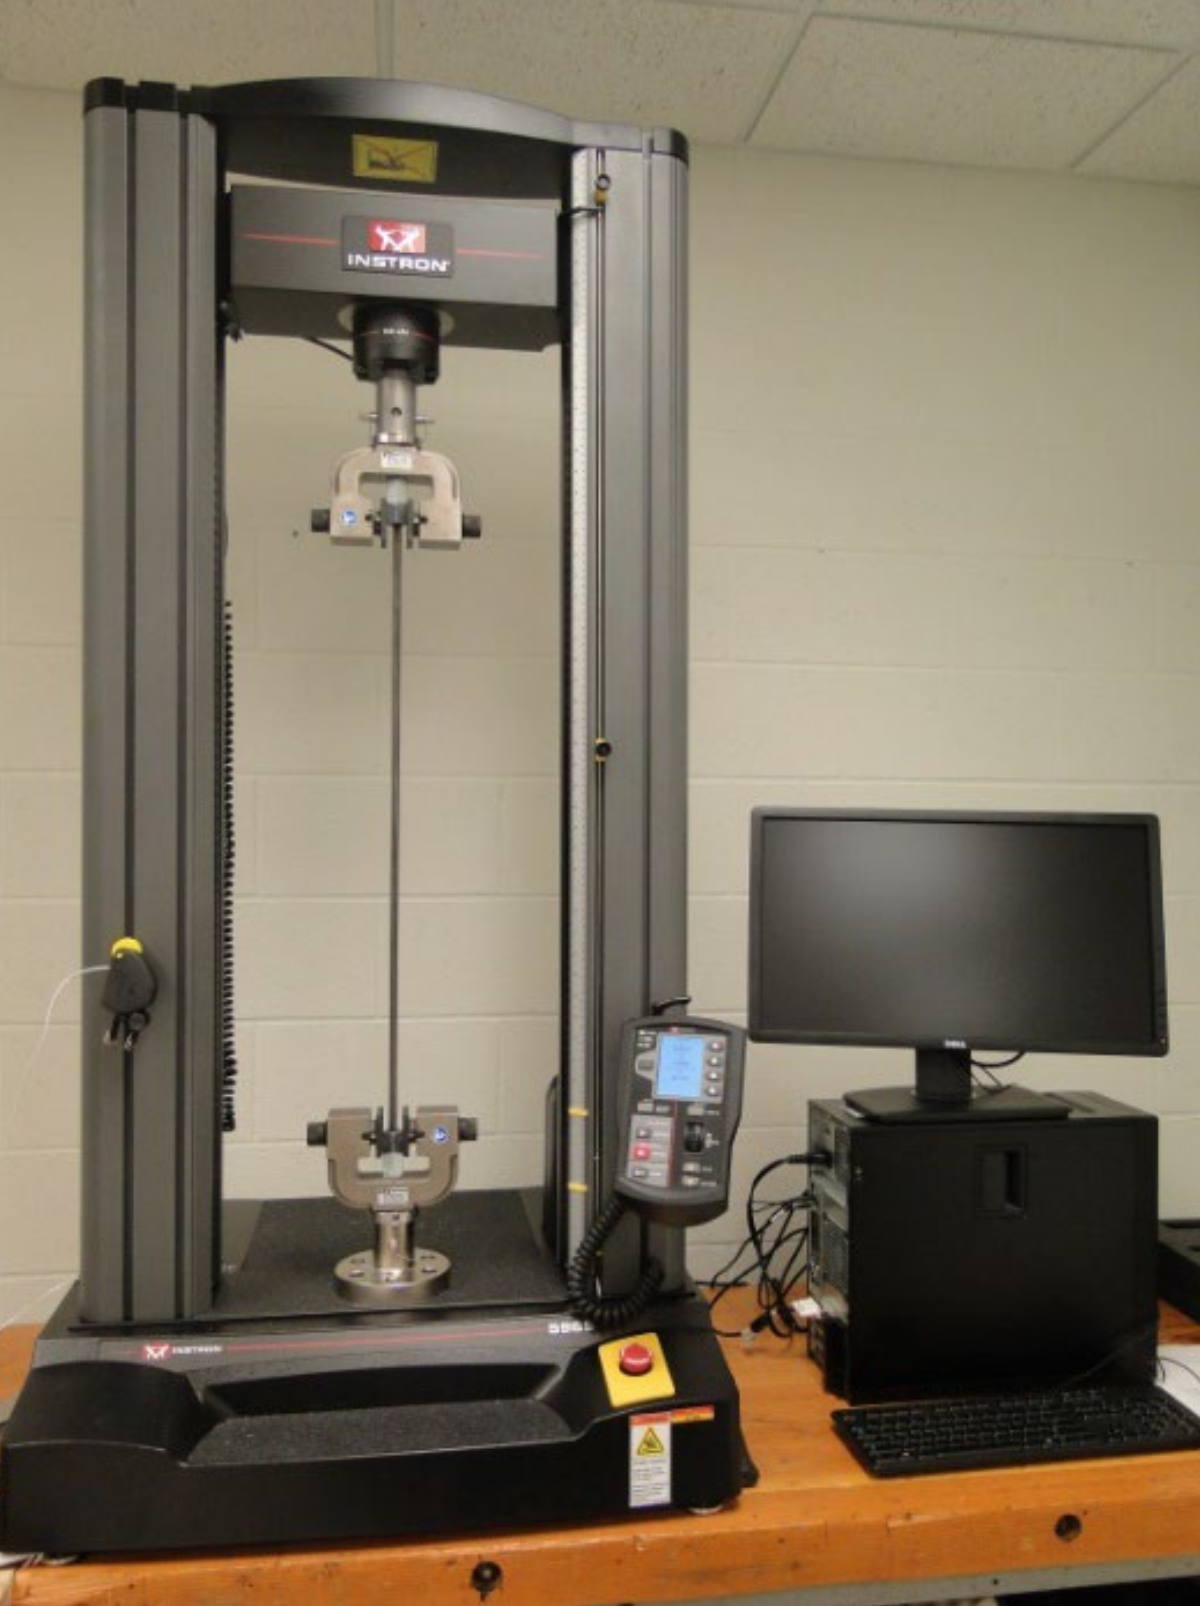
\includegraphics[width=1.0\textwidth]{images/instron_1}
		\caption{The Instron loaded with a metal column specimen.}
		\label{fig:instron_1}
    \end{minipage}\hfill
    \begin{minipage}{0.45\textwidth}
        \centering
		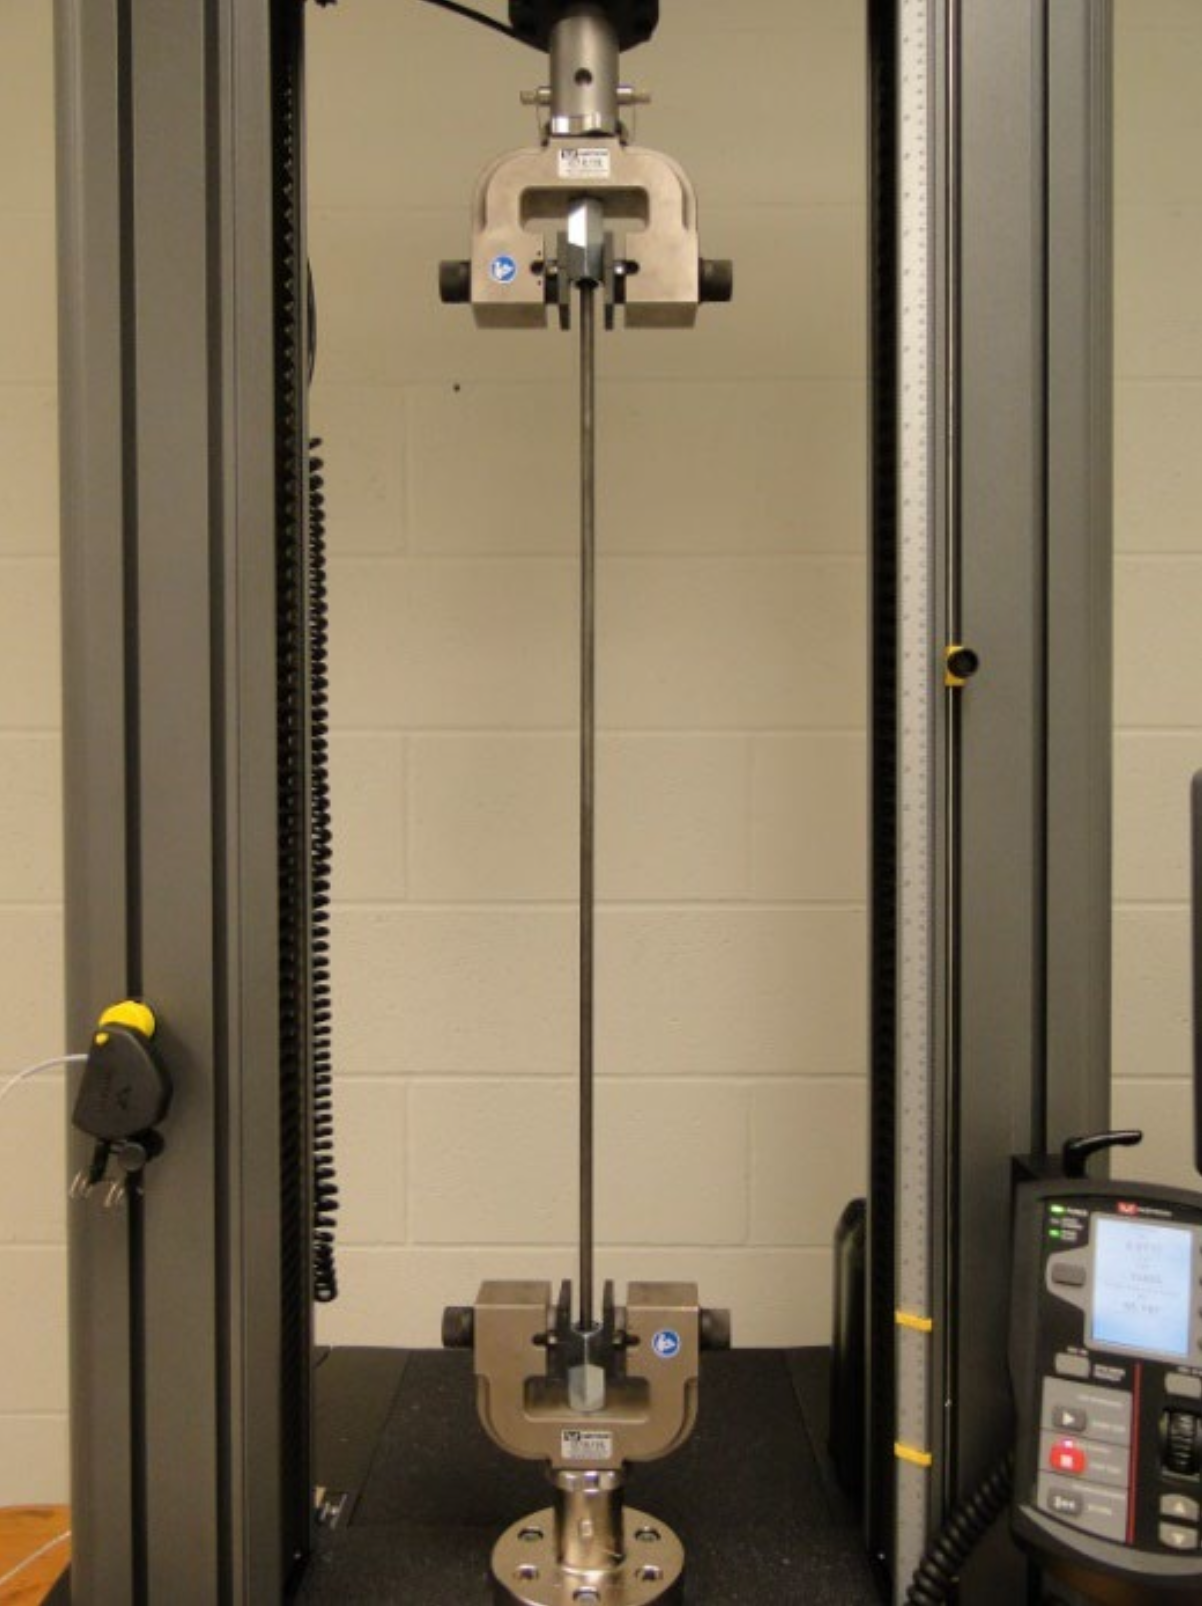
\includegraphics[width=1.0\textwidth]{images/instron_2}
		\caption{The Instron configured for a column buckling test.}
		\label{fig:instron_2}
    \end{minipage}
\end{figure}

\begin{figure}[htbp]
	\centering
	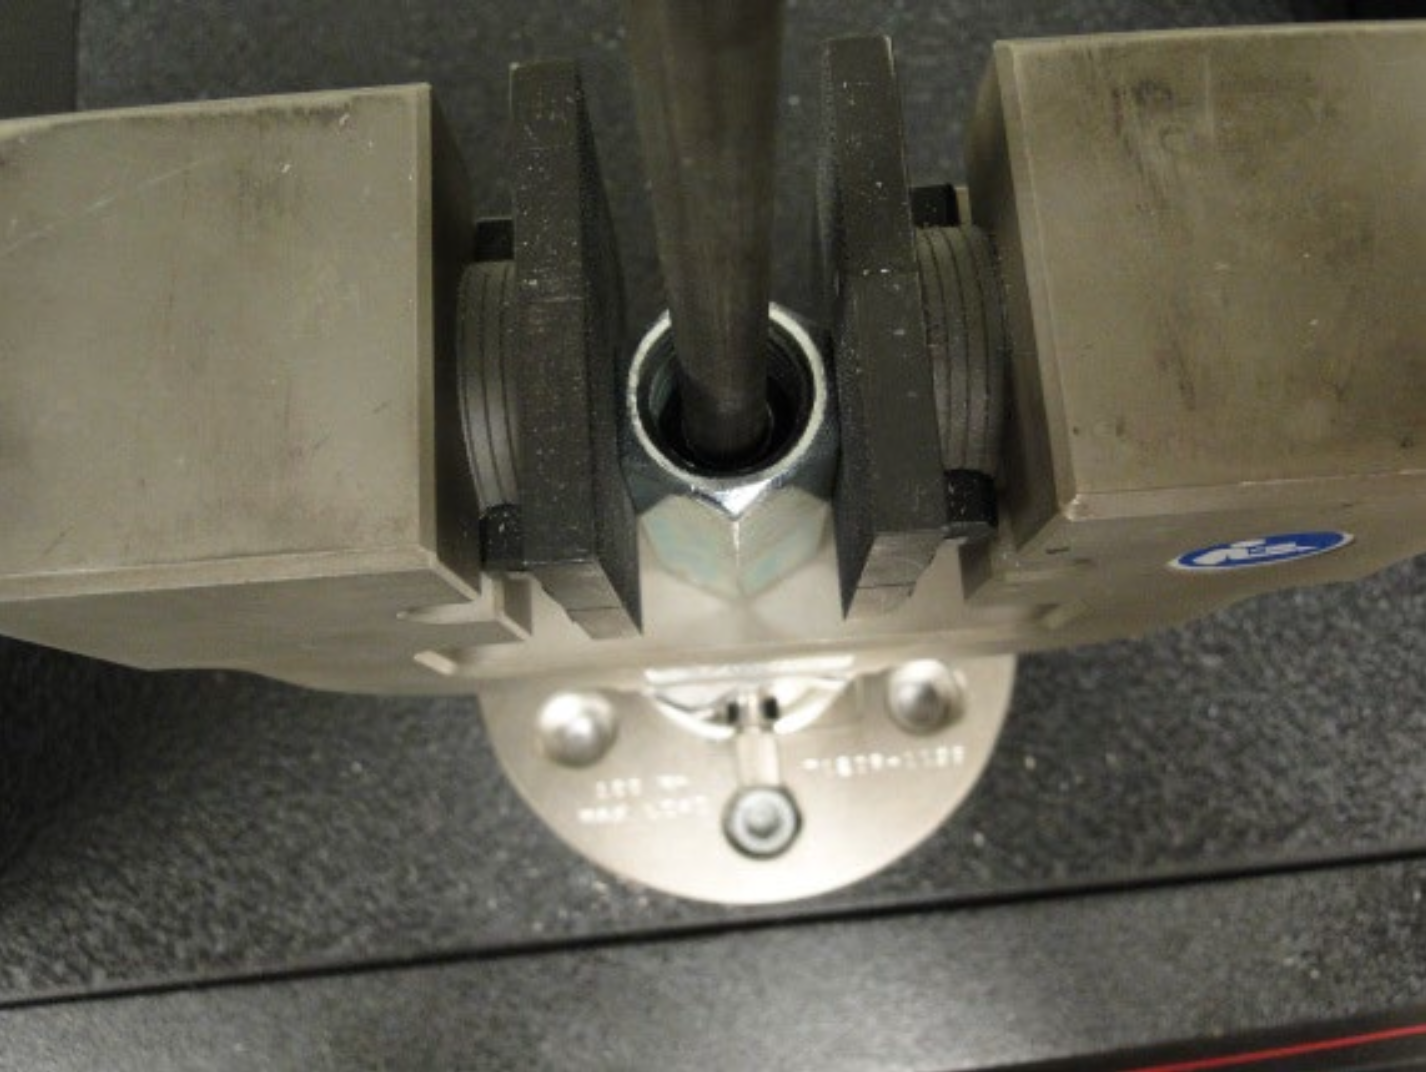
\includegraphics[width=4in]{images/socket}
	\caption{A close-up of the socket used to hold the specimens in the Instron machine.}
	\label{fig:socket}
\end{figure}

\section{Procedures} \label{procedures}
Insert the specimen into the Instron. While the specimen is in the socket, but still unloaded, zero the Instron to reset all the measurements. Using the fine adjustment knob, decrease the gaps between the specimen ends and the sockets until the specimen is loaded with \qty{5}{lb}. Record the distance between the sockets or between the socket and the grip.

Visually align the column with a vertical marker behind the column. Increase the compressive force with the fine adjustment knob at a rate of one click per second. Once the specimen ``jolts'' or buckles away from the visual marker, note and record the current force. Unload the specimen. Repeat this whole procedure for all five specimen.

\section{Data} \label{data}
The critical load and slenderness ratio data from prelab is tabulated in Table \ref{tbl:prelab}

\begin{table}[!htbp]
\caption{Theoretical critical loads and slenderness ratios.}
\begin{center}
	\begin{tabular}{|c|c|c|c|c|}
		\hline
		Configuration&$P_{cr}$ [\unit{lb}]&$\frac{L}{\rho}$\\
		\hline
		\num{1}&\num{106.5}&\num{320.0}\\
		\hline
		\num{2}&\num{142.8}&\num{415.7}\\
		\hline
		\num{3}&\num{60.98}&\num{480.0}\\
		\hline
		\num{4}&\num{95.28}&\num{384.0}\\
		\hline
		\num{5}&\num{124.4}&\num{336.0}\\
		\hline
	\end{tabular}
\end{center}
\label{tbl:prelab}
\end{table}

Data collected from the experiment is tabulated in Table \ref{tbl:data}.

\begin{table}[!htbp]
\caption{Data collected from the lab. Specimen one through three were tested twice whereas specimens four through five were tested three times. $P_\text{cr}$ is the theoretical critical load.}
\begin{center}
	\begin{tabular}{|c|c|c|c|c|}
		\hline
		Specimen ID&Length [\unit{in}]&$P_\text{cr,avg}$ [\unit{in}]&$P_\text{cr}$ [\unit{lb}]&Error\\
		\hline
		\num{1}&\num{30}&\num{-133}&\num{-106.5}&\qty{24.9}{\percent}\\
		\hline
		\num{2}&\num{29.5}&\num{-126}&\num{-147.7}&\qty{14.7}{\percent}\\
		\hline
		\num{3}&\num{30}&\num{-54.8}&\num{-60.98}&\qty{10.1}{\percent}\\
		\hline
		\num{4}&\num{24}&\num{-91.7}&\num{-92.58}&\qty{0.915}{\percent}\\
		\hline
		\num{5}&\num{27.5}&\num{-102}&\num{-148.1}&\qty{31.4}{\percent}\\
		\hline
	\end{tabular}
\end{center}
\label{tbl:data}
\end{table}

\section{Analysis} \label{analysis}
In the test for configuration two, we successfully predicted the column would buckle about the axis that runs parallel to the \qty{1}{in} edge of the column. The moment of inertia---calculated using Equation \ref{eqn:I}---about this axis is \qty{1.302e-3}{in^4} versus \qty{2.083e-2}{in^4} for the perpendicular axis. Since the moment of inertia about the former axis is lower than the moment of inertia about the latter axis, the resistance to bending is lower about the former axis and will buckle first.
\begin{align}
	I&=\frac{1}{12}bh^3\label{eqn:I}
\end{align}
The buckling jolt for specimen one was the hardest to see of the five specimens. It was very easy to see the jolt in specimen three. The jolt in specimen four was comparable to specimen three, and still significantly easier to spot than specimen one. We suspect part of the reason specimen one was so difficult to see was due to its low slenderness ratio, $\frac{L}{\rho}$, shown in Table \ref{tbl:prelab}, caused by its thicker diameter.

The buckling jolt for specimen five was more difficult to observe than in specimens two through four, but it was slightly easier than spotting the jolt in specimen one. Specimens one and five had the smallest slenderness ratio and the buckling jolt was very difficult to detect. From this, we observe that columns with low slenderness ratios are less susceptible to buckling than columns with high slenderness ratios.

This is further substantiated by the relative error calculations. The specimens that obviously buckled or jolted (specimens two through four) had less than \qty{15}{\percent} relative error whereas specimens one and five both had very high relative error. It is easier to calculate the critical load on a beam that is highly susceptible to buckling---\eg specimens two through four---whereas detecting exactly when the critical load has been surpassed on beams that are not sensitive to buckling---\eg specimens one and five---is very difficult with the naked eye as it is more of a gradual transition than a jolt.

Additionally, the theoretical critical load may have impacted our ability to observe the buckling jolt. Each tick of the fine position knob increased the compressive force by \qtyrange{5}{10}{lb}. In specimen three, this is approximately a \qty{12}{\percent} increase relative to the theoretical critical load. In specimen five, this is approximately a \qty{5.1}{\percent} increase relative to the theoretical critical load. For specimens with higher critical loads, the relative increase in compression stress for each tick of the fine position knob is lower causing sudden jolts or buckling effects to be less noticeable.

The largest source of error in this experiment comes from the subjective observation of the buckling jolt. This buckling is measured in terms of millimeters and is very difficult to see according to the naked eye. Additionally, what classifies as a jolt is also subjective. To address this subjectivity with a rectangular columns, we suggest placing a displacement needle at the theoretical point of maximum buckling for the given length and end-configuration and recording the displacement and compression force simultaneously. The buckling jolt could easily be identified in post analysis of the data. For cylindrical columns, two displacement needles could be positioned at \ang{90} to recording the displacement in two dimensions. Again, once the magnitude of the displacement surpassed a threshold, \eg \qty{1}{\mm}, the corresponding compressive force would be the critical load.

Besides the subjective measurement of the jolt, the mechanical properties of each material, especially Young's Modulus, $E$, will vary slightly depending on the specimen. Additionally, the fine position needle increased the compressive force by \qtyrange{5}{10}{lb} each tick, which dramatically limits the resolution of $P_\text{cr}$. We could address this error by using the aforementioned displacement needles in combination with an automated Instron test that linearly increased the compressive force per unit time.

To maximize the critical load of the steel specimens in a pivot-pivot end-configuration by adjusting the cross-sectional dimensions---but keeping the area constant---we must first recall definitions derived in prelab. The definition of critical load, $P_\text{cr}$ is defined in Equation \ref{eqn:P_cr}.
\begin{align}
	P_\text{cr}&=\frac{\pi^2Ebh^3}{12L^2}\label{eqn:P_cr}
\end{align}
where $E$ is the Young's Modulus of the specimen in units of pressure, $b$ and $h$ are the cross-sectional dimensions in units of length, and $L$ is the effective length of the column. In theoretical calculations, $b$ and $h$ can be chosen arbitrarily. But in reality, the column will always buckle according to the weakest configuration of $b$ and $h$.

For example, if the cross-sectional dimensions of a column are \qtyproduct{1x2}{in}, the theoretical value of $P_\text{cr}$ may be either of the following:
\begin{align*}
	P_\text{cr}&=\frac{2\pi^2E}{3L^2}\\
	P_\text{cr}&=\frac{\pi^2E}{6L^2}
\end{align*}
In reality, however, the column will always buckle based on the value of $P_\text{cr}$ lowest in magnitude, \eg $P_\text{cr}=\frac{\pi^2E}{6L^2}$. Generalizing this statement based on Equation \ref{eqn:P_cr}, we say that in reality, $h$ will always be less than or equal to $b$, \ie $h\le{}b$.

Since we have an additional constraint on the cross-sectional dimensions, we can define a system of equations to determine the cross-sectional dimensions that result in the maximum critical load, $P_\text{cr,max}$. Equation \ref{eqn:area_constraint} is based on the constraint that the area of the column must remain constant.
\begin{align}
	b&=\frac{A}{h}\label{eqn:area_constraint}
\end{align}
where $A$ is the constant cross sectional area of the column. Substituting Equation \ref{eqn:area_constraint} into Equation \ref{eqn:P_cr}, we find that
\begin{align}
	P_\text{cr}&=\frac{\pi^2EAh^2}{12L^2}\label{eqn:subsituted_P_cr}
\end{align}
Since $E$, $A$, and $L$ are all constant, $P_\text{cr}$ increases as $h$ increases, and therefore, $P_\text{cr,max}$ occurs when $h$ is at its maximum value. As noted prior, $h$ is bounded above by $b$, and hence, $P_\text{cr,max}$ occurs when $h=b$. Geometrically, if $h=b$, the column is a square.

To maximize $P_\text{cr}$ then, we let $b=h=\sqrt{A}$. The calculations for this configuration, shown below, are based on the material parameters and the area of the steel specimen three.
\begin{align*}
	b=h&=\sqrt{A}\\
	&=\sqrt{\pi(\qty{0.125}{in})^2}\\
	&=\qty{0.2216}{in}
\end{align*}
\begin{align*}
	P_\text{cr,rect}&=\frac{\pi^2Ebh^3}{12L^2}\\
	&=\frac{\pi^2(\qty{29000e3}{psi})(\qty{0.2216}{in})(\qty{0.2216}{in})^3}{12(\qty{30}{in})^2}\\
	&=\qty{63.86}{lb}
\end{align*}
\begin{align*}
	\sigma_\text{cr,rect}&=\frac{P_\text{cr,rect}}{bh}=\frac{\pi^2Eh^2}{12L^2}\\
	&=\frac{\pi^2(\qty{29000e3}{psi})(\qty{0.2216}{in})^2}{12(\qty{30}{in})^2}\\
	&=\qty{1.301}{ksi}
\end{align*}
\begin{align*}
	\left(\frac{L}{\rho}\right)_\text{rect}&=\frac{2L}{H}\sqrt{3}\\
	&=\frac{2(\qty{30}{in})}{(\qty{0.2216}{in})}\sqrt{3}\\
	&=\num{469.1}
\end{align*}

When designing a column, there are a number of factors that need to be considered. First and foremost is the column's critical load, $P_\text{cr}$ and its resistance to buckling, \ie the slenderness ratio, $\frac{L}{\rho}$. If these constraints are not satisfied, the column and the structure its supporting may fail. Some structures may handle buckling whereas other structures may be considered unsafe if any buckling has occurred. Additionally, the end-configuration of the column can make a significant difference on the critical load and maximum loads.

Some other design constraints that are less related to the material properties: If conserving cost is a primary constraint, minimizing the cross-sectional area may be desirable. If it is likely a structure will fail or if it is designed to fail, using a rectangular column is better than a cylindrical column since the mode, direction, and characteristics of the failure can easily be predicted. Lastly, in some scenarios, it may be important for technicians or auditors to observe degradation in the columns. If this is the case, then using a column that buckles or fails gradually is preferable to a column that fails suddenly or unexpectedly.

\section{Conclusion} \label{conclusion}
In general, the measured critical loads matched the theoretical critical load. For specimen two, we successfully predicted the direction which the column would buckle by calculating the moments of inertia. The highest errors were measured for specimen one and specimen five which we suspect is due to the low slenderness ratio---it was very difficult to see the ``jolt'' in specimen one and specimen five, and specimen five consistently buckled early.

We learned what material and geometric properties affect the strength and effectiveness of a column and how to calculate the theoretical critical loads and slenderness ratios.
\end{document}
